%Dokumentklasse

%draft als optionohne bilder für bessere performance
%\documentclass[a4paper,12pt,]{scrreprt}

%normal mit Bildern
\documentclass[
a4paper,
11pt,
draft=True]
{scrartcl}

%Section als Chapter
\RedeclareSectionCommand[%
%beforeskip = -1sp plus -1sp minus -1sp,% kleinster negativer Wert, um den Absatzeinzug nach der Überschrift zu verhindern.
afterskip = 1.5 \baselineskip plus -1sp minus 1sp,
font = \Huge,
]{section}

\usepackage[left= 3cm,right = 3cm, bottom = 3cm,top = 3cm]{geometry}
%\usepackage[onehalfspacing]{setspace}

% ============= Packages =============
% Dokumentinformationen
\usepackage[
pdftitle={Praktikum - Umwelttechnik},
pdfsubject={},
pdfauthor={Roman-Luca Zank},
pdfkeywords={},	
%Links nicht einrahmen
hidelinks
]{hyperref}

%nur Text zum prüfen des Umfangs

% Standard Packages
%\usepackage[bottom]{footmisc}
\usepackage[utf8]{inputenc}
\usepackage[ngerman]{babel}

\usepackage[T1]{fontenc}
%\usepackage{helvet}
\usepackage{rotating}

%\renewcommand{\familydefault}{\sfdefault}

\usepackage{graphicx}
\graphicspath{{img/}}
\usepackage[table]{xcolor}
\setlength\arrayrulewidth{0.8pt}
\usepackage{mhchem}
\usepackage{fancyhdr}
\usepackage{lmodern}
\usepackage{color}
\usepackage[bottom]{footmisc}
\usepackage{setspace}\usepackage{threeparttable}
%==================================================================
%\begin{threeparttable} 
%	\begin{tabular}{|l|c|r|} 
%		\hline 
%		A & B & C \\
%		\hline
%		1 & 2 & 3 \tnote{1} \\
%		\hline
%	\end{tabular} 
%	\begin{tablenotes}\footnotesize 
%		\item[1] Prognose 2003 
%	\end{tablenotes}
%====================================================================
\usepackage{placeins}
\usepackage{booktabs}
\usepackage{caption}
\usepackage[list=true]{subcaption}
\usepackage[longtable]{multirow}
\usepackage{tikz}
\usepackage{pgfplots}
\pgfplotsset{/pgf/number format/use comma}
\usepackage{lastpage}
%\usepackage{ulem}
\usepackage{mathtools}
\usepackage{adjustbox}
\usetikzlibrary{patterns}
\usepackage{pdfpages}
\usepackage{colortbl}

%Einheitenpackage
\usepackage{siunitx}  
\sisetup{	locale = DE, 
	per-mode=fraction,
	inter-unit-product=\ensuremath{\cdot},
	detect-weight = true,
	quotient-mode=fraction
}
%neue Einheiten definieren
\DeclareSIUnit\xyz{xyz}	
\DeclareSIUnit\rpm{rpm}	
\DeclareSIUnit\mws{mWS}	
\DeclareSIUnit\degrees{^\circ}	
\DeclareSIUnit\volp{V\%}
\DeclareSIUnit\mpp{m\%}
\DeclareSIUnit\mmWS{mmWS}
\DeclareSIUnit\cmt{\raiseto{3}\meter}
\DeclareSIUnit\sqm{\raiseto{2}\meter}

%Automatisch cdot statt *
\DeclareMathSymbol{*}{\mathbin}{symbols}{"01}


%Tabelle
\usepackage{tabularx}
\usepackage{tabulary}

%nur letzte Zeile der Gleichung nummerieren
\makeatletter
\def\Let@{\def\\{\notag\math@cr}}
\makeatother

%angepasster \today Command
\newcommand{\leadingzero}[1]{\ifnum #1<10 0\the#1\else\the#1\fi}
\newcommand{\todayDE}{\leadingzero{\day}.\leadingzero{\month}.\the\year}

% zusätzliche Schriftzeichen der American Mathematical Society
\usepackage{amsfonts}
\usepackage{amsmath}

%Abkürzungsverzeichnis
\usepackage{acronym}

%kein Abstand bei neuem Kapitel vom Seitenanfang
%\vspace*{2.3\baselineskip} = ORIGINAL
%\renewcommand*{\chapterheadstartvskip}{\vspace*{.0\baselineskip}}

%nicht einrücken nach Absatz
\setlength{\parindent}{0pt}

\urlstyle{same}


% ============= Kopf- und Fußzeile =============
\pagestyle{fancy}
%
\lhead{}
\chead{}
\rhead{}%\slshape }%\leftmark}
%%
\lfoot{}
\cfoot{}
\rfoot[{\thepage\ of \pageref*{LastPage}}]{Seite \thepage\ von \pageref*{LastPage}}
%%
\renewcommand{\headrulewidth}{0pt}
\renewcommand{\footrulewidth}{0pt}
%\renewcommand{\chapterpagestyle}{fancy}

%Fußnotelinie
%\let\footnoterule

%Fußnote mit Klammer
\renewcommand*{\thefootnote}{(\arabic{footnote})}

%Abb. statt Abbildung
\addto\captionsngerman{%
	\renewcommand{\figurename}{Abb.}%
	\renewcommand{\tablename}{Tab.}%
}

% ============= Package Einstellungen & Sonstiges ============= 
%Besondere Trennungen
%\hyphenation{De-zi-mal-tren-nung}
\usepackage[none]{hyphenat}
\hyphenpenalty=5000
\tolerance=5000
\providecommand\phantomsection{}

\usepackage{mathtools}


% ============= Dokumentbeginn =============

\begin{document}
%Seiten ohne Kopf- und Fußzeile sowie Seitenzahl
\pagestyle{empty}

%\begin{center}
\begin{tabular}{p{\textwidth}}


\begin{center}

\includegraphics[scale=0.75]{logos.jpg}\\
\end{center}


\\

\begin{center}
\LARGE{\textsc{
Protokoll \\
Thermische Verfahrenstechnik I\\
}}
\end{center}

\\

%\begin{center}
%\large{Fakultät für Muster und Beispiele \\
%der Hochschule Musterhausen \\}
%\end{center}
%
%\\
\begin{center}
	\textbf{\Large{Bestimmung des Wärmeübergangskoeffizienten}}
\end{center}

\\ \\
%\begin{center}
%zur Erlangung des akademischen Grades\\
%Bachelor of Engineering
%\end{center}


%\begin{center}
%vorgelegt von
%\end{center}

\begin{center}
\Large{\textbf{Teilnehmer:}} \\ 
\end{center}
\begin{center}
\large{Willy Messerschmidt \\
	Roman-Luca Zank} \\
\end{center}


\\ \\ \\ \\ \\ \\

\begin{center}
\begin{tabular}{lll}
\large{\textbf{Gruppe:}} & & \large{J}\\
&&\\
\large{\textbf{Protokollführer:}} & & \large{Roman-Luca Zank}\\
&&\\
\large{\textbf{Datum der Versuchsdurchführung:}}&& \large{Online}\\
&&\\
\large{\textbf{Abgabedatum:}}&& \large{\today}
\end{tabular}
\end{center}

\\ \\ \\ \\ \\ \\ \\ \\ \\ \\ \\ \\
\large{Merseburg den \today}

\end{tabular}
\end{center}


%\include{14_danksagungen}

%\include{15_zusammenfassung}

% Beendet eine Seite und erzwingt auf den nachfolgenden Seiten die Ausgabe aller Gleitobjekte (z.B. Abbildungen), die bislang definiert, aber noch nicht ausgegeben wurden. Dieser Befehl fügt, falls nötig, eine leere Seite ein, sodaß die nächste Seite nach den Gleitobjekten eine ungerade Seitennummer hat. 
\cleardoubleoddpage

% Pagestyle für Titelblatt leer
\pagestyle{empty}

%Seite zählen ab
\setcounter{page}{0}

%Titelblatt
\begin{center}
\begin{tabular}{p{\textwidth}}


\begin{center}

\includegraphics[scale=0.75]{logos.jpg}\\
\end{center}


\\

\begin{center}
\LARGE{\textsc{
Protokoll \\
Thermische Verfahrenstechnik I\\
}}
\end{center}

\\

%\begin{center}
%\large{Fakultät für Muster und Beispiele \\
%der Hochschule Musterhausen \\}
%\end{center}
%
%\\
\begin{center}
	\textbf{\Large{Bestimmung des Wärmeübergangskoeffizienten}}
\end{center}

\\ \\
%\begin{center}
%zur Erlangung des akademischen Grades\\
%Bachelor of Engineering
%\end{center}


%\begin{center}
%vorgelegt von
%\end{center}

\begin{center}
\Large{\textbf{Teilnehmer:}} \\ 
\end{center}
\begin{center}
\large{Willy Messerschmidt \\
	Roman-Luca Zank} \\
\end{center}


\\ \\ \\ \\ \\ \\

\begin{center}
\begin{tabular}{lll}
\large{\textbf{Gruppe:}} & & \large{J}\\
&&\\
\large{\textbf{Protokollführer:}} & & \large{Roman-Luca Zank}\\
&&\\
\large{\textbf{Datum der Versuchsdurchführung:}}&& \large{Online}\\
&&\\
\large{\textbf{Abgabedatum:}}&& \large{\today}
\end{tabular}
\end{center}

\\ \\ \\ \\ \\ \\ \\ \\ \\ \\ \\ \\
\large{Merseburg den \today}

\end{tabular}
\end{center}
 %Prokolle
%\begin{center}
\begin{tabular}{p{\textwidth}}


\begin{center}

\includegraphics[scale=0.75]{img/logos.jpg}\\
\end{center}


\\

\begin{center}
\LARGE{\textsc{
Recherche \\
Rückgewinnung von Ammoniak aus Industrieabwässern\\
}}
\end{center}

%\begin{center}
%\large{Fakultät für Muster und Beispiele \\
%der Hochschule Musterhausen \\}
%\end{center}
%
%\\
 \\
 
\begin{center}
\textbf{\Large{Seminararbeit in Medienrecherche}}
\end{center}

\begin{center}
	\large{im WiSe 2019}
\end{center}
 \\
%\begin{center}
%zur Erlangung des akademischen Grades\\
%Bachelor of Engineering
%\end{center}


\begin{center}
\large{vorgelegt von}
\end{center}
\\


\begin{center}
\Large{\textbf{Roman-Luca Zank}} \\
\end{center}

\begin{center}
3. Semester \\
Chemie- und Umwelttechnik \\
\end{center}


\begin{center}
\begin{tabular}{lll}
	\textbf{E-Mail:} & & romanzank@mail.de\\
	\textbf{Matrikelnummer:} & &25240\\
	\textbf{Adresse:} & &Platz der Bausoldaten 2, Zimmer 224\\
	\textbf{Ort:} & &06217 Merseburg\\
	&& \\
	\textbf{Prüfer:} & & Dr. Frank  Baumann\\
\end{tabular}
\end{center}

\\ \\ \\ \\ \\
\large{Merseburg, \today}

\end{tabular}
\end{center}
 %Seminar-/Abschlussarbeit

% Pagestyle für Rest des Dokuments
\pagestyle{fancy}

%Inhaltsverzeichnis
\tableofcontents
\thispagestyle{empty}

%Inhalt
%
%Verzeichnis aller Bilder
\label{sec:bilder}
\listoffigures
\addcontentsline{toc}{chapter}{Abbildungsverzeichnis}
\thispagestyle{empty}

%Verzeichnis aller Tabellen
\label{sec:tabellen}
\listoftables
\addcontentsline{toc}{chapter}{Tabellenverzeichnis}
\thispagestyle{empty}



%%Abkürzungsverzeichnis
%\setlength{\columnsep}{20pt}
%\twocolumn
%\addchap{Nomenklatur}
%\label{sec:abkurzung}
%\begin{acronym}
%\acro{kf}[$\text{k}_\text{f}$]{Durchlässigkeitsbeiwert}
%\acro{t}{Durchlaufzeit}
%\acro{tm}[$\text{t}_\text{m}$]{Mittlere Durchlaufzeit}
%\acro{V}{Volumen}
%\acro{h}{Höhe der Wassersäule}
%\acro{Q}{Volumenstrom}
%\acro{l}{Durchströmte Länge}
%\acro{A}{Grundfläche}
%\acro{d}{Durchmesser}
%
%\end{acronym}
%\subsubsection{Aufrufen einer Abkürzung}
%\acs{rT}
%\begin{verbatim}
%\acs{Abkürzung}
%\end{verbatim}

%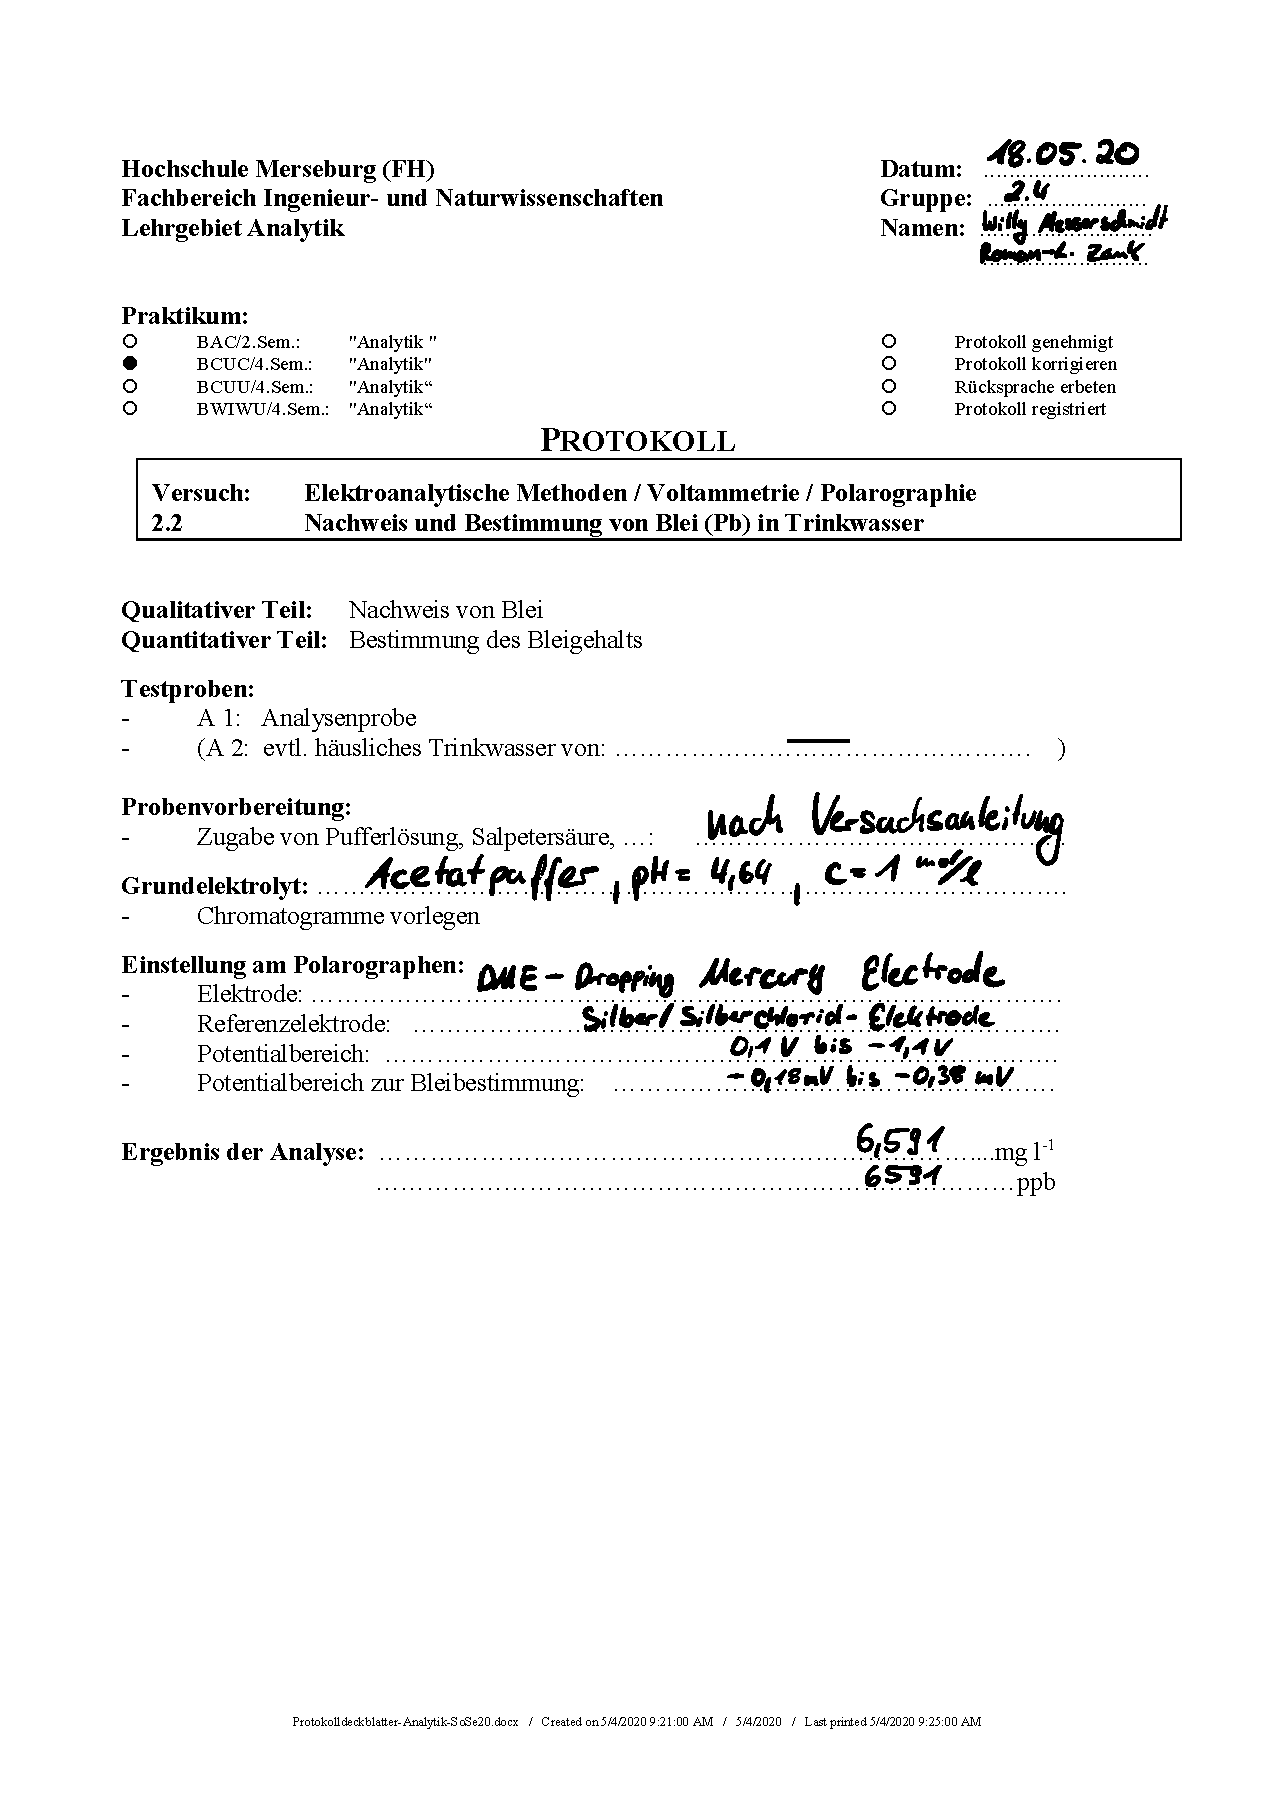
\includepdf[]{Deckblatt}
\pagebreak
\section{Einleitung}
\label{sec:einleitung}
Im folgenden Protokoll werden generierte Messdaten zum Versuch \textit{WÜK} ausgewertet. Ziel ist es mithilfe der erklärenden Videos zum Praktikum und Mittels der gegebenen Messdaten den Wärmeübergangskoeffizient $\alpha_L$ für turbulente Luftströmungen zu bestimmen. Dafür werden  drei verschiedene Rohre unter unterschiedlichen Volumenströmen der Luft untersucht. Die Wärmeübertragung mit Wasser erfolgt  in diesem Versuch mittels Gegenstrom.
Darüber hinaus sind, mittels \textsc{Nußelt}-Zahl $Nu$ und der \textsc{Nußelt}-Parameter $a$ und $b$, Bewertungen zur Wärmeübertragung der verschiedenen Rohre und Volumenströme abzugeben.







\section{Theoretische Grundlagen}
\label{sec:theorie}

Grundlage für den Versuch stellte die Wärmeübertragung am Rohr da. So lässt sich der übertragende Wärmestrom über die spezifische Wärmekapazität, dem Massenstrom, sowie aus der Differenz zwischen eingehender und ausgehender Temperatur des Stromes.
\begin{flalign}
 	\dot{Q} &= \dot{m}*c_p*\Delta T\\
 	\dot{Q} &= \dot{m}*c_p*(T_\omega-T_\alpha)
\end{flalign}

\begin{flalign}
	\Delta T_{_{\ln}}	&=  \frac{\Delta T_A-\Delta T_B}{\ln\left(\frac{\Delta T_A}{\Delta T_B}\right)}\\[1mm]
	\dot{Q} 	 &= U_a *A*\Delta T_{_{\ln}}\\
	U_a				&= \frac{\dot{Q}}{\Delta T_{_{\ln}}}
\end{flalign}

\begin{flalign}
	U_a		&= \left(\frac{1}{\alpha_i}+\sum\frac{d}{\lambda}+\frac{1}{\alpha_a}\right)^{-1}\\
	\alpha_i &=\left(\frac{1}{U_a}-\sum\frac{d}{\lambda}+\frac{1}{\alpha_a}\right)^{-1}
\end{flalign}

\begin{flalign}
	d_H \, (\text{Rohr})	&= D_i-d_a
\end{flalign}

\begin{flalign}
	Re	&= \frac{d*w}{\nu}
\end{flalign}

\begin{flalign}
		Pr	&= \frac{c_p*\nu*\rho}{\lambda}
\end{flalign}

\begin{flalign}
	Nu_{\text{ideal}}	&= 0,023*\left(Re^2*Pr\right)^{0,4}
\end{flalign}
\begin{flalign}
	Nu 	&= \frac{\alpha*d}{\lambda}\\[1mm]
	\alpha	&=  \frac{Nu*\lambda}{d}
\end{flalign}

\begin{flalign}
	a	&= e^{\ln(Nu)}
\end{flalign}
\begin{flalign}
	b &= f'\left(\ln(Re^2*Pr),\ln(Nu)\right)
\end{flalign}

\textcolor{red}{Stoff und Rohrdaten}

%\newpage
\section{Geräte und Chemikalien}
\label{sec:geraete}

\textbf{Geräte:}
\begin{itemize}
\item Trockenofen Mettler-Toledo DO-302
\item Waage
\item Titrator T50, \textsc{Karl-Fischer}-Titrator (Fa. Mettler)
\item Computer mit Software \textsc{LabX}
\item Mikroliterspritze
\end{itemize}

\vspace*{5mm}

\textbf{Proben/Chemikalien:}
\begin{itemize}
\item \textsc{Karl-Fischer}-Reagenz (Einkomponentig)
\item deionisiertes Wasser
\item Isopropanol (2-Propanol)
\item Polyamid

\end{itemize}







\newpage
\section{Durchführung}
\label{sec:durchfuerung}

Der Versuch der Flammpunktprüfung erfolgte in diesem Fall nach der \linebreak Pensky-Martens-Methode in einem geschlossenen Tiegel nach der Norm DIN EN ISO 2719.\linebreak
Hierfür wurden die Proben jeweils in den sauberen Tiegel der automatische Messapperatur gefüllt und ein Wert für den zu erwartenden Flammpunkt eingegeben. Das Messgerät beginnt infolgedessen die etappenweise Prüfung des Flammpunkts mittels Glühdrahts unter konstanter Temperaturerhöhung. Ist der Flammpunkt um thermische Sensoren detektiert worden, aufgrund eines kurzen Temperaturmaximums durch die Entflammung, wird die Messung beendet.\\
Für die Prüfung der Weinprobe auf ihren Volumenanteil mittel Flammpunktprüfung wird eine 
Rein-Ethanol-Wasser-Mischung mit der genau dem angegebenen an Ethanol (\SI{12}{\volp}) hergestellt und diese miteinander verglichen.


%\newpage
\section{Ergebnisse und Berechnungen}
\label{sec:ergebnisse}

\subsection{Allgemeine Daten}
Aus den geometrischen Daten und den gemessenen Volumenströmen lassen sich die Daten der Tabellen \ref{tab:strom_reihe} und \ref{tab:strom_para} bestimmen. Diese sind relevant für weiterführende Berechnungen in den folgenden Abschnitten.

% Table generated by Excel2LaTeX from sheet 'Daten'
\begin{table}[h!]
	\renewcommand*{\arraystretch}{1.2}
	\centering
	\rowcolors{2}{gray!25}{white}
	\caption{Strömungsrelevante Größen der Reihenschaltung}
	\label{tab:strom_reihe}
	\resizebox{15cm}{!}{
		\begin{tabulary}{1.2\textwidth}{CCCCC}
			\hline
			\textbf{Strom}&\textbf{Fläche} $\left[\si{\sqm}\right]$&\textbf{hydr. Durchmesser} $\left[\si{\meter}\right]$&\textbf{Volumenstrom} $\left[\si{\cmt\per\second}\right]$&\textbf{Geschwindigkeit} $\left[\si{\meter\per\second}\right]$ \\
			\hline
			warm&\SI{7,85E-05}{}&\SI{0,010}{}&\SI{1,32E-04}{}&\SI{1,68}{}\\
			kalt	&\SI{6,83E-05}{}&\SI{0,003}{}&\SI{8,63E-05}{}&\SI{1,26}{}\\
			\hline			
		\end{tabulary}
	}
\end{table}%
\FloatBarrier

% Table generated by Excel2LaTeX from sheet 'Daten'
\begin{table}[h!]
	\renewcommand*{\arraystretch}{1.2}
	\centering
	\rowcolors{2}{gray!25}{white}
	\caption{Strömungsrelevante Größen der Parallelschaltung}
	\label{tab:strom_para}
	\resizebox{15cm}{!}{
		\begin{tabulary}{1.2\textwidth}{CCCCC}
			\hline
			\textbf{Strom}&\textbf{Fläche} $\left[\si{\sqm}\right]$&\textbf{hydr. Durchmesser} $\left[\si{\meter}\right]$&\textbf{Volumenstrom} $\left[\si{\cmt\per\second}\right]$&\textbf{Geschwindigkeit} $\left[\si{\meter\per\second}\right]$ \\
			\hline
			warm&\SI{7,85E-05}{}&\SI{0,010}{}&\SI{1,45E-04}{}&\SI{1,85}{}\\
			kalt	&\SI{6,83E-05}{}&\SI{0,003}{}&\SI{1,45E-04}{}&\SI{2,12}{}\\
			\hline			
		\end{tabulary}
	}
\end{table}%
\FloatBarrier

\subsection{Messdaten und Temperaturprofile}
Zunächst werden allgemein die theoretischen Messdaten in den Tabellen \ref{tab:messung_reihe} und \ref{tab:messung_para} für die Reihen- und Parallelschaltung dargestellt.

\begin{table}[h!]
		\centering
	\rowcolors{2}{gray!25}{white}
	\caption{Temperatur- und Druckmesswerte für die Reihenschaltung}
	\resizebox{7cm}{!}{
	\begin{tabulary}{\textwidth}{L|C|C}
		\textbf{Messstelle} & \textbf{Temperatur} $\left[\si{\celsius}\right]$& \textbf{Druck} $\left[\si{\bar}\right]$\\
		\hline
		$T_{\alpha,\text{warm}}$ & 55,38 & 1,030\\
		$T_{\text{zw1},\text{warm}}$  & 46,58 & 0,690  \\
		$T_{\text{zw2},\text{warm}}$  & 46,56 & 0,500\\
		$T_{\omega,\text{warm}}$  & 32,73 & 0,215 \\
		\hline
		$T_{\alpha,\text{kalt}}$  & 16,10 & 2,300\\
		$T_{\text{zw2},\text{kalt}}$   & 36,71 & 0,900  \\
		$T_{\text{zw1},\text{kalt}}$   & 36,75 & 1,300   \\
		$T_{\omega,\text{kalt}}$ & 49,68 & 0,065 \\
	\end{tabulary}%
}
	\label{tab:messung_reihe}%
\end{table}%
\FloatBarrier
\,
\begin{table}[h!]
	\centering
	\rowcolors{2}{gray!25}{white}
	\caption{Temperatur- und Druckmesswerte für die Parallelschaltung}
	\resizebox{7cm}{!}{
	\begin{tabulary}{\textwidth}{L|C|C}
		\textbf{Messstelle} & \textbf{Temperatur} $\left[\si{\celsius}\right]$& \textbf{Druck} $\left[\si{\bar}\right]$\\
		\hline
		$T_{1,\alpha,\text{warm}}$ & 55,54 & 0,200\\
		$T_{1,\omega,\text{warm}}$  & 30,71 & 0,152  \\
		$T_{2, \alpha,\text{warm}}$  & 55,63 & 0,310\\
		$T_{2,\omega,\text{warm}}$  & 31,52 & 0,300 \\
		\hline
		$T_{1,\alpha,\text{kalt}}$ & 16,21 & 1,530\\
		$T_{1,\omega,\text{kalt}}$  & 38,41 & 0,400  \\
		$T_{2, \alpha,\text{kalt}}$  & 16,30 & 1,580\\
		$T_{2,\omega,\text{kalt}}$  & 39,83 & 0,507 \\
	\end{tabulary}%
	}
	\label{tab:messung_para}%
\end{table}%
\FloatBarrier

Die Verläufe der Temperaturen für die einzelnen Wärmetauscher ergibt, zeigt sich in Abbildung \ref{dia:temp_profil}.

\vspace*{-7mm}

\begin{figure}[h!]
	\begin{center}
		\resizebox{0.7\textwidth}{!}{
			\begin{tikzpicture}[trim axis left, trim axis right]
			\begin{axis}[
			grid,
			axis lines = left,
			width = 15cm,
			height = 9cm,
			xmin = 0,
			xmax = 15,
			ymin = 0,
			ymax = 60,
			ytick = {0,5,...,60},
			xtick = {0,1,2,...,15},
			ylabel={Temperatur in \si{\celsius}},
			%y label style={at={(0,0.5)}},
			xlabel={Rohrabschnitt in \si{\meter}},
			legend style={at={(0.75,0.95)},anchor=west},
			%	y dir = reverse,
			]			
			%Warm Reihe
			\addplot [color=red, mark=*] coordinates{(0,55.38) (7.5,46.58) (7.51,46.56) (15, 32.73)};
			
			%Kalt Reihe
			\addplot [color=blue, mark=*] coordinates{(0,49.68) (7.5,36.75) (7.51,36.71) (15, 16.10)};
			
			%Warm Wü1
			\addplot [color=red, mark=square, dotted] coordinates{(0,55.54) (7.5, 30.71)};
			
			%Warm WÜ2
			\addplot [color=red, mark=triangle, dashed] coordinates{(0,55.63) (7.5, 31.52)};
			
			\addplot [color=blue, mark=square, dotted] coordinates{(0,38.41) (7.5, 16.21)};
			
			\addplot [color=blue, mark=triangle, dashed] coordinates{(0,39.83) (7.5, 16.30)};
			
			
			\legend{Warm (Reihe), Kalt (Reihe), Warm (WÜ1 | Parallel), Warm (WÜ2 | Parallel), Kalt (WÜ1 | Parallel), Kalt (WÜ2 | Parallel)}
			\end{axis}
			\end{tikzpicture}
		}
		\caption{Temperaturverläufe der Wärmetauscher}
		\label{dia:temp_profil}
	\end{center}
\end{figure}
\FloatBarrier

\subsection{Wärmeströme}
Um zu prüfen in welchem Maße der Wärmeübergang stattfindet, werden die Wärmeströme der verschiedenen Schaltungen untersucht. Dabei wird der gemessene Volumenstrom in der Berechnung mit einem Korrekturvolumenstrom angepasst. Daraus ergibt sich jeweils für die aufgenommene bzw. abgegebene Wärme ein korrigierter Volumenstrom. Genauere Beschreibungen hierzu finden sich in der Theorie unter Abschnitt \ref{sec:theorie}.\\
Zur Vereinfachung der Berechnungen wird eine konstante, spezifische Wärmekapazität angenommen. Die Dichten, welche für Berechnungen der Massenströme und den daraus resultierenden Wärmeströmen nötig sind, werden über die jeweils kälteste Temperatur des warmen bzw. kalten Stromes berechnet.\\
Die berechneten Werte finden sich in den Tabellen \ref{tab:warme_reihe} und \ref{tab:warme_para}.

% Table generated by Excel2LaTeX from sheet 'GegenstromReihe neu'
\begin{table}[h!]
	\renewcommand*{\arraystretch}{1.2}
	\centering
	\rowcolors{2}{white}{gray!25}
	\caption{Berechnete Wärmeströme und Korrekturvolumenstrom für die Reihenschaltung}
	\resizebox{15cm}{!}{
	\begin{tabulary}{1.2\textwidth}{C|CC|C|CC|C}
		\hline
		\textbf{System} & $\boldsymbol{Q_{ab}} \, \left[\si{\kilo \watt}\right]$ & $\boldsymbol{Q_{auf}} \, \left[\si{\kilo \watt}\right]$& $\boldsymbol{\dot{V}_{korr}} \, \left[\si{\cmt \per \second}\right]$& $\boldsymbol{Q_{ab, korr}} \, \left[\si{\kilo \watt}\right]$&$\boldsymbol{Q_{auf, korr}} \, \left[\si{\kilo \watt}\right]$ & $\boldsymbol{\Delta Q_{korr}} \, \left[\si{\kilo \watt}\right]$\\
		\hline
		WÜ1   & 7,58  & 7,44  &\SI{ -9,70E-07 }{}& 7,53  & 7,53  & 0,00 \\
		WÜ2   & 4,83  & 4,67  & \SI{-1,71E-06}{} & 4,76  & 4,76  & 0,00 \\
		\hline
		Gesamt & 12,42 & 12,13 & \SI{-1,24E-06}{} & 12,30 & 12,30 & 0,00 \\
		\end{tabulary}%
	}
	\label{tab:warme_reihe}%
\end{table}%
\FloatBarrier

% Table generated by Excel2LaTeX from sheet 'GegenstromReihe neu'
\begin{table}[h!]
	\renewcommand*{\arraystretch}{1.2}
	\centering
	\rowcolors{2}{white}{gray!25}
	\caption{Berechnete Wärmeströme und Korrekturvolumenstrom für die Parallelschaltung}
	\resizebox{15cm}{!}{
		\begin{tabulary}{1.2\textwidth}{C|CC|C|CC|C}
			\hline
			\textbf{System} & $\boldsymbol{Q_{ab}} \, \left[\si{\kilo \watt}\right]$ & $\boldsymbol{Q_{auf}} \, \left[\si{\kilo \watt}\right]$& $\boldsymbol{\dot{V}_{korr}} \, \left[\si{\cmt \per \second}\right]$& $\boldsymbol{Q_{ab, korr}} \, \left[\si{\kilo \watt}\right]$&$\boldsymbol{Q_{auf, korr}} \, \left[\si{\kilo \watt}\right]$ & $\boldsymbol{\Delta Q_{korr}} \, \left[\si{\kilo \watt}\right]$\\
			\hline
			WÜ1   & 7,50  & 6,72  &\SI{ -8,00E-06 }{}& 7,09 & 7,09 & 0,00 \\
			WÜ2   & 7,28 & 7,12  & \SI{-1,64E-06}{} & 7,20  & 7,20  & 0,00 \\
			\hline
			Gesamt   & 14,78 & 13,84  & \SI{-9,64E-06}{} & 14,29  & 14,29  & 0,00 \\
			\hline
		\end{tabulary}%
	}
	\label{tab:warme_para}%
\end{table}%
\FloatBarrier
\newpage
\subsection{Leistungen und Wärmeübertragungsparameter}
Um nun die Effizienz der Anlage besser beschreiben zu können, wird der transportierte Wärmestrom in ein Verhältnis zur elektrischen Leistung einer Kreiselpumpe mit 80\% Wirkungsgrad gesetzt. Diese Kreiselpumpe fördert die jeweilige Flüssigkeit durch das System.\\
Über die dimensionslosen Kennzahlen $Re$, $Pr$ und $Nu$ lassen sich nun die Wärmeübertragungsparameter $\alpha $ und $U$ berechnen. Über diese Werte lässt sich der Wärmeübertragungsprozess unabhängig von der Geometrie miteinander vergleichen. Zur Vereinfachung der Rechnungen wird die Wärmeleitfähigkeit vom Stahlrohr mit \SI{15}{\watt\per\meter \per\kelvin} angenommen. Die Wärmeleitfähigkeit des Fluides, sowie die Viskosität werden jedoch als Funktion von der Temperatur eingerechnet.\\
Die Ergebnisse dieser Rechnungen finden sich in den Tabellen \ref{tab:leistung_reihe} und \ref{tab:leistung_para} wieder und lassen sich mithilfe der theoretischen Grundlagen nachvollziehen.
\begin{table}[h!]
	\centering
	%\rowcolors{3}{gray!25}{white}{gray!10}
	\caption{Berechnete Leistungen, dimensionslose Kennzahlen und \linebreak Wärmeübertragungsparameter der Reihenschaltung}
	\resizebox{15cm}{!}{
	\begin{tabulary}{1.55\textwidth}{L|C|CCC||CCC|CC}
		\hline
		\textbf{System} & $\boldsymbol{\Delta p} \, \left[\si{\bar}\right]$ & $\boldsymbol{P_{Pumpe}} \, \left[\si{\kilo \watt}\right]$ &  $\boldsymbol{P_{Elektrisch}} \, \left[\si{\kilo \watt}\right]$& $\boldsymbol{Q/P_{Elektrisch}}$ & \textbf{Re} & \textbf{Pr}& \textbf{Nu} & $\boldsymbol{\alpha}  \, \left[\si{\kilo \watt \per \sqm \per \kelvin}\right]$ & $\boldsymbol{U} \, \left[\si{\watt \per \meter\per \kelvin}\right]$ \\
		\hline
		WÜ1 warm & 0,29  & \SI{3,76E-03}{} & \SI{4,70E-03}{}3 & 1602  & \SI{2,20E+04}{} & 5,13  & \SI{131,9}{} & 8,14  & \multirow{2}{*}{31,13}  \\
		WÜ1 kalt & 20,61 &\SI{ 1,78E-01 }{}&\SI{ 2,22E-01}{} & 34    &\SI{ 3,41E+03}{} & 7,87  & \SI{35,2 }{}& 6,93  &  \\
		\hline
		WÜ2 warm & 0,35  & \SI{4,66E-03 }{}& \SI{5,83E-03 }{}& 817   & \SI{2,87E+04}{} & 3,80  & \SI{144,5}{} & 9,20  & \multirow{2}{*}{34,98} \\
		WÜ2 kalt & 12,93 & \SI{1,12E-01}{} &\SI{ 1,40E-01 }{}& 34    & \SI{5,39E+03}{} & 4,68  & \SI{41,2}{} & 8,57  &  \\
		\hline
		Gesamt warm & 0,82  & \multirow{2}{*}{\SI{3,00E-02
			}{}}&  \multirow{2}{*}{\SI{3,76E-02}{}} & \multirow{2}{*}{328}   & -&- & -& - & -\\
		Gesamt kalt & 2,24  & & &    & -&- & -& - & -\\
		\hline
	\end{tabulary}%
}
	\label{tab:leistung_reihe}
\end{table}%
\vspace*{-5mm}
\begin{table}[h!]
	\centering
%	\rowcolors{2}{gray!25}{white}
	\caption{Berechnete Leistungen, dimensionslose Kennzahlen und \linebreak Wärmeübertragungsparameter der Parallelschaltung}
	\resizebox{15cm}{!}{
		\begin{tabulary}{1.55\textwidth}{L|C|CCC||CCC|CC}
			\hline
			\textbf{System} & $\boldsymbol{\Delta p} \, \left[\si{\bar}\right]$ & $\boldsymbol{P_{Pumpe}} \, \left[\si{\kilo \watt}\right]$ &  $\boldsymbol{P_{Elektrisch}} \, \left[\si{\kilo \watt}\right]$& $\boldsymbol{Q/P_{Elektrisch}}$ & \textbf{Re} & \textbf{Pr}& \textbf{Nu} & $\boldsymbol{\alpha}  \, \left[\si{\kilo \watt \per \sqm \per \kelvin}\right]$ & $\boldsymbol{U} \, \left[\si{\watt \per \meter\per \kelvin}\right]$ \\
			\hline
			WÜ1 warm & 0,06 & \SI{4,21E-04}{} & \SI{5,27E-04}{}& 13464  & \SI{1,16E+04}{} & 5,39  & \SI{80,62}{} & 4,96  & \multirow{2}{*}{23,97} \\
			WÜ1 kalt & 2,20 &\SI{ 1,60E-02 }{}&\SI{ 2,00E-02}{} & 354    &\SI{ 2,87E+03}{} & 7,83  & \SI{30,57}{}& 6,02  &  \\
			\hline
			WÜ2 warm & 0,01  & \SI{7,26E-05 }{}& \SI{9,08E-05 }{}& 79320   & \SI{1,18E+04}{} & 5,28  & \SI{81,10}{} & 4,99 & \multirow{2}{*}{24,08} \\
			WÜ2 kalt & 1,07 & \SI{7,79E-03}{} &\SI{ 9,74E-03 }{}& 739    & \SI{2,87E+03}{} & 7,83  & \SI{30,62}{} & 6,03 &  \\
			\hline
			Gesamt warm & 0,07  & \multirow{2}{*}{\SI{2,43E-02
				}{}}&  \multirow{2}{*}{\SI{3,04E-02}{}} & \multirow{2}{*}{471}   & -&- & -& - & -\\
			Gesamt kalt & 3,28 & & &    & -&- & -& - & -\\
			\hline
		\end{tabulary}%
}
	\label{tab:leistung_para}
\end{table}%



\newpage
\section{Diskussion}
\label{sec:diskussion}
Beginnend mit den Temperaturprofilen der Wärmetauscher für die Reihen- und Parallelschaltung werden an dieser Stelle die Messergebnisse diskutiert und bewertet. Die in der Abbildung \ref{dia:temp_profil} dargestellten Temperaturverläufe, welche über den Rohrabschnitt aufgetragen wurden,  geben erste Indizien zur Bewertung der beiden Fahrweisen. Es zeigt sich, dass die Temperaturverläufe für den parallelen Betrieb deutlich steiler zulaufen als für die Reihenschaltung. Zu erkennen ist ebenfalls, dass die Temperaturdifferenzen der Parallelschaltung größer sind, als die der Reihenschaltung. Somit lässt sich die Vermutung aufstellen, dass die Parallelschaltung die effizientere Wärmeübertragung für die jeweils eingestellten Volumina liefert. Jedoch sollte beachtet werden, dass für beide Verfahren unterschiedliche Volumenströme gefahren werden. Somit kann anhand dieses Diagramms lediglich die Fahrweise mit den entsprechenden Betriebsparametern verglichen werden. Es gibt jedoch keine Auskunft über den Vergleich von Reihen- und Parallelschaltung.\\

Anhand der Wärmeströme lassen sich nun beide Fahrweisen quantitativ unterscheiden. Die Korrektur der Volumenströme ist hierbei notwendig und gibt Auskunft über den Fehler der Messungen am jeweiligen System. An dieser Stelle zeigt sich, dass über die Parallelschaltung, in Bezug auf die Menge an übertragener Wärme,  effizienter erscheint als die Reihenschaltung. Doch dass lediglich mehr Wärme übertragen wird, gibt noch keine Aussage über die Effizienz des Schaltung. Es lässt sich jedoch sagen, dass offensichtlich in der Parallelschaltung mehr Wärme übertragen und somit abgeführt werden kann, als es für die Reihenschaltung der Fall ist.\\

Zieht man in die Betrachtung nun auch die Wirtschaftlichkeit der jeweiligen Fahrweise mit ein, so setzt man die übertragene Wärmemenge in ein Verhältnis zur benötigen elektrischen Leistung für die Förderung des Fluides. Wirtschaftlichkeit bedeutet in diesem Fall, dass maximal viel Wärme übertragen wird, für einen minimalen Einsatz an elektrischer Leistung für die Kreiselpumpe. Demnach ist das Ziel möglichst hohe Werte für dieses Verhältnis zu erreichen. Es zeigt sich, dass die Werte für die Parallelschaltung deutlich wirtschaftlicher erscheinen als die Reihenschaltung, aufgrund der höheren Menge an übertragenen Wärme über den auszugleichenden Druckverlust. Im Gesamtaufbau überzeugt die Parallelschaltung mit einem Ergebnis, welches um 30\% besser ist, als das der Reihenschaltung.
So besticht die Parallelschaltung unter diesem Aspekt, sowohl für die einzelnen Wärmeübertrager, als auch im Gesamtsystem für diesen Versuchsaufbau. \\

Vergleicht man nun zuletzt die Wärmeübergangs- sowie die Wärmedurchgangskoeffizienten zeigt sich die Fahrweise der Reihenschaltung als effektiver. Erkennbar ist dies daran, dass für jeden betrachteten Wärmetauscher der Wert für die übertragene Fläche pro Quadratmeter und Kelvin in der Reihenschaltung höher ist. Auch der Wärmedurchgang, welcher die übertragene Wärme pro Meter Rohrleitung und Kelvin angibt, ist für diesen Versuchsaufbau für die Reihenschaltung größer. Ein Vergleich der Wärmedurchgangskoeffizienten in \mbox{Diagramm \ref{dia:durchng}} verdeutlicht nochmals grafisch, dass die Wärmetauscher im Reihenbetrieb effizienter arbeiten.

\begin{figure}[h!]
	\begin{center}
		\resizebox{0.8\textwidth}{!}{
			\begin{tikzpicture}
			\begin{axis}[
			width  = 0.85*\textwidth,
			height = 7cm,
			major x tick style = transparent,
			ybar=2*\pgflinewidth,
			bar width=14pt,
			ymajorgrids = true,
			ylabel = {$U \, \left[\si{\watt \per \meter\per\kelvin}\right]$},
			symbolic x coords={WÜ1,WÜ2},
			xtick = data,
			scaled y ticks = false,
			enlarge x limits=0.25,
			ymin=0,
			legend cell align=left,
			legend style={
				at={(1,1.05)},
				anchor=south east,
				column sep=1ex
			}
			]
			%Reihenschaltung
			\addplot[style={black,fill=black,mark=none}]
			coordinates {(WÜ1, 31.13) (WÜ2,34.98)};
			
			%Paralaleschaltung
			\addplot[style={gray,fill=gray,mark=none}]
			coordinates {(WÜ1,23.97) (WÜ2,24.08)};
			
			
			\legend{Reihenschaltung, Parallelschaltung}
			\end{axis}
			\end{tikzpicture}
		}
		\caption{Grafischer Vergleich der Wärmedurchgangskoeffizienten}
		\label{dia:durchng}
	\end{center}
\end{figure}
\FloatBarrier
\newpage
Schlussendlich lässt sich sagen, dass für die gegebenen Betriebsparameter die Parallelschaltung in ihrer Effizienz gegenüber der Reihenschaltung überzeugt. Gerade in Bezug auf die Wirtschaftlichkeit hat die Reihenschaltung keine überzeugenden Argumente für den Betrieb hervorgebracht. Jedoch ist die Reihenschaltung in Bezug auf den Wärmeübergangsprozess effizienter als die Parallelschaltung. Da im Regelfall die benötigte Pumpleistung für den Parallelbetrieb, aufgrund von Strömungswiderständen, größer wäre und sich somit auch der wirtschaftliche Faktor ändern würde, ist es sinnvoller eine Reihenschaltung vorzuziehen. Aus den Ergebnissen des theoretischen Versuches für dieses Protokoll ist jedoch laut dem wirtschaftlichen Aspekt die Parallelschaltung vorzuziehen.

Der berechnete Wärmeverlust entspricht mit den in Gleichung \eqref{gl:Energie-eingesetzt} berechneten \SI{637,5}{\watt} 52\% der Heizleistung. Dies ist aufgrund der vielen un-isolierten Bereiche an der Kolonne plausibel.

%\section{Fehlerbetrachtung}
\label{sec:fehler}
Für die Fehlerbetrachtung ist davon auszugehen, dass jegliche Messeinrichtungen die Messwerte mit Fehlern in bestimmten Toleranzen aufnehmen. Weiterhin sind Vereinfachungen für die auswertenden Berechnungen angenommen worden, welche die ausgewerteten Ergebnisse ebenfalls verfälschen. Die vorliegenden Ergebnisse sind demnach nur eine Näherung an den realen Zustand. Dennoch sind sie ausreichend um die qualitativen Unterschiede zwischen Reihen- und Parallelschaltung aufzuzeigen.\\
Um einen Teil der fehlerbehafteten Größen für die einzelnen Wärmetauscher zu quantifizieren bzw. die Wärmeströme entsprechend zu korrigieren, wurde für diesen Versuch ein Korrekturvolumenstrom eingeführt. Für die jeweilige Schaltung und den jeweiligen Wärmetauscher sind diese Korrekturvolumenströme im Diagramm \ref{dia:korrrek} aufgetragen. Dabei ist zu erkennen, dass der Betrag des Korrekturvolumenstroms für den \mbox{Wärmeübertrager 1} am höchsten hervorsticht. Dies sollte bei der Bewertung der berechneten Daten berücksichtigt werden.\\
Weiterhin sind Vereinfachungen getroffen worden, dass sich beispielsweise die Volumenströme in der Parallelschaltung gleichmäßig aufteilen, sowie dass für bestimmte, temperaturabhängige Größen Näherungsgleichungen genutzt wurden.

\begin{figure}[h!]
	\begin{center}
		\resizebox{0.8\textwidth}{!}{
			\begin{tikzpicture}
			\begin{axis}[
			width  = 0.85*\textwidth,
			height = 7cm,
			major x tick style = transparent,
			ybar=2*\pgflinewidth,
			bar width=14pt,
			ymajorgrids = true,
			ylabel = {$\left|\Delta \dot{V}\right|\, \left[\si{\cmt\per \second}\right]$},
			symbolic x coords={WÜ1,WÜ2},
			xtick = data,
			%scaled y ticks = false,
			enlarge x limits=0.25,
			ymin=0,
			ymax=0.00001,
			legend cell align=left,
			legend style={
				at={(1,1.05)},
				anchor=south east,
				column sep=1ex
			}
			]
			%Reihenschaltung
			\addplot[style={black,fill=black,mark=none}]
			coordinates {(WÜ1, 9.7E-07) (WÜ2,1.71E-06)};
			
			%Paralaleschaltung
			\addplot[style={gray,fill=gray,mark=none}]
			coordinates {(WÜ1,8.00E-06) (WÜ2,1.64E-06)};
			
			
			\legend{Reihenschaltung, Parallelschaltung}
			\end{axis}
			\end{tikzpicture}
		}
		\caption{Grafischer Vergleich der Korrekturvolumenströme}
		\label{dia:korrrek}
	\end{center}
\end{figure}
\FloatBarrier
\newpage

Auffallend für die Fehlerbetrachtung ist noch, dass die Messwerte für diesen theoretischen Versuch eine höhere Pumpleistung für die Reihen- als für Parallelleistung erfordert wird. Dies erscheint nicht als sinnvoll, da gerade durch die Aufteilung, die Lenkung und wieder Zusammenführung der Strömungen im Parallelbetrieb ein höherer Druckverlust entstehen würde als in der Reihenschaltung. Die Reihenschaltung erfordert nämlich keine Umlenkung oder Aufteilung des Fluidstroms.\\

Im Endeffekt lässt sich sagen, dass der Versuch erneut durchgeführt werden sollte, um die Ergebnisse dieses Versuches zu überprüfen. Weiterhin sollten beide Fahrweisen unter den selben Volumenströmen gefahren werden, da ein Vergleich sonst nur bedingt sinnvoll erscheint, wenn man lediglich die Schaltungen der Wärmetauscher überprüfen möchte.

%%\section*{Anhang}
\addcontentsline{toc}{section}{Anhang}
%\label{sec:anhang}
 
 
 
 

%%Praktikumsskript, Modul ………, Versuch …….., Prof. Musterprof. 
%DIN 12345, Jahr der Veröffentlichung 
%Link der Internetseite, Zugriffsdatum 
%Buchtitel, Autor, Verlag, Veröffentlichungsjahr 

%Literaturverzeichnis Bücher
\bibliography{Literatur}
\bibliographystyle{unsrtdin}
\addcontentsline{toc}{section}{Literaturverzeichnis}

%\chapter*{Eidesstattliche Erklärung}
\label{erklaerung}
Hiermit versichere ich, die vorliegende Seminararbeit selbstständig und nur unter Verwendung der von mir angegebenen Quellen und Hilfsmittel verfasst zu haben. Sowohl inhaltlich als auch wörtlich entnommene Inhalte wurden als solche kenntlich gemacht. Die Arbeit hat in dieser oder vergleichbarer Form noch keinem anderem Prüfungsgremium vorgelegen. \\
\\[1.5cm]
Datum:	\hrulefill\enspace Unterschrift: \hrulefill
\\[3.5cm]
\addcontentsline{toc}{chapter}{Selbstständigkeitserklärung}

\end{document}
